\documentclass{article}
\usepackage{mathmag}

\usepackage{amsmath,amsthm}
\usepackage{graphicx}
\usepackage{hyperref}
\usepackage{url}
\usepackage{amsfonts}

\usepackage{multicol}


% NOTE mathmag.sty calls the text fonts. For this template we are using times.sty
% from the standard LaTeX distribution.

%% IF YOU HAVE FONTS INSTALLED you can use these math fonts to more
%% closely approximate the final product.
%\usepackage{mtpro2}
%\usepackage{mathtime}

\theoremstyle{theorem}
\newtheorem{theorem}{Theorem}

\theoremstyle{definition}
\newtheorem*{definition}{Definition}
\newtheorem*{remark}{Remark}

\allowdisplaybreaks

\makeatletter
\@addtoreset{footnote}{page}
\makeatother

%%%%%%%%%%%%%%%%%%%%%%%%%%%%%%%%%%%%%%%%%%%%%%%%%%
\begin{document}

\title{Segregation Surfaces}

\author{Author Name\\               %%%% Leave ALL of these as is in your initial submission
\scriptsize affiliation line 1\\    %%%% to allow for double blind reviewing.
affiliation line 2\\                %%%% They should be filled in when you are submitting
email address}                      %%%% your final manuscript.

\maketitle

\noindent Over the past half century, social scientists have devised a clever assortment of tools to measure the nature and extent of segregation. \cite{harrisjohnson18} Usually, a segregation measurement takes the form of a number, or \textit{index}, which quantifies the isolation and clustering of groups defined by race, income, education, or other factors. Numerical indices are handy because they can give us ways to track changes in a neighborhood over time, and they allow for comparisons among different regions.

However, segregation usually takes place on a map, not on a number line. Numerical summary statistics alone are limited when it comes to finding geometric patterns in two-dimensional data. In this note, we use some familiar ideas from third-semester calculus to extend the machinery behind some commonly-used segregation indices. We will see how segregation can be represented by a surface, and how the geometric properties of these surfaces reveal ways that our cities and towns are divided.

\section{Numerical measures of segregation.}

In order to define a segregation measure, we assume that we have data describing the population within particular geographic region, including the locations of where people live. For simplicity, we will regard the population as being split into two groups $A$ and $B$, where $B$ is the complement of $A$ (e.g., white/non-white, above/below median income). Most of the measures we consider below can be extended to more than two groups.

One of the earliest measures of segregation to become widely adopted is the \textit{index of dissimilarity} of Duncan and Duncan. \cite{duncan55} The definition of this index depends on a partition of region in question; typically, this partition is defined by census tracts or block groups. For subset $i$ of this partition, let $a_i$ be the population of group $A$, and let $b_i$ be the population of group $B$. The index of dissimilarity $D$ is then given by summing the differences of the proportions of each group living in each subset.

\begin{equation}
  D = \frac{1}{2} \sum_i \left\lvert \frac{a_i}{\lvert A \rvert} - \frac{b_i}{\lvert B \rvert} \right\rvert
\end{equation}

If our two groups were evenly distributed, we would expect each of the $n$ subsets to contain $\frac{1}{n}$ of the total population of each, giving an index of $D = 0$. On the other hand, if our region were completely segregated, each subset would would contain zero of one group, so the above summation would simply tally up the proportions of each, resulting in $D = 1$.

The index of dissimilarity has two glaring weaknesses. First, it is highly sensitive to how the subsets are defined. A different allocation of census tracts could result in a different value of $D$. Second, it suffers from the so-called ``checkerboard problem.'' \cite{morrill91}. Figure~\ref{fig:checkerboard} shows three different segregation patterns. Suppose that $|A| = |B|$ and that each subset contains the same number of residents. For a fixed proportion $p$, suppose that $p$ each shaded subset is from group $A$ and $1-p$ is from group $B$, while $p$ of each non-shaded region is from group $B$ and $1-p$ from group $A$. It is easy to check that $D = \lvert 2p-1 \rvert$ in all three cases, even though the first pattern seems objectively more segregated than the third.

\begin{figure}\centering
  \includegraphics[width=4in]{checkerboard.pdf}
  \caption{Three different segregation patterns with the same index of dissimilarity.}
  \label{fig:checkerboard}
\end{figure}

To address these two weaknesses, Sullivan and Wong \cite{sullivanwong07} propose a generalization of $D$ using surfaces. Let $a(x,y)$ and $b(x,y)$ be two-dimensional probability density functions describing the distribution of groups $A$ and $B$, respectively, in our region $R$. The segregation index $S$ is then defined as

\begin{equation}
  S = 1 - \frac{V_\cap}{V_\cup},
\end{equation}

where

\begin{equation}
  V_\cap = \iint_R \min(a, b) \, dA \quad \text{ and } \quad V_\cup = \iint_R \max(a,b) \, dA.
\end{equation}

If groups $A$ and $B$ are identically distributed, then $V_\cap$ will equal $V\cup$, resulting in $S = 0$. However, more segregation will tend to reduce the volume $V_\cap$ under both surfaces relative to the total volume $V_\cup$, yielding values of $S$ closer to~1.

For example, consider the segregation patterns in Figure~\ref{fig:checkerboard}, letting the region $R$ be the square $[0,1] \times [0,1]$, and suppose that $0.5 < p \leq 1$. Suppose that $a(x,y)$ is a piecewise constant density function, taking the value $2p$ in the shaded regions and $2(1-p)$ in the non-shaded regions. Similarly, let $b(x,y)$ take the value $2(1-p)$ in the shaded regions and $2p$ in the non-shaded regions. Then $V_\cap = 2(1-p)$ and $V_\cup = 2p$, giving $S = (2p-1)/p$ for all three patterns.

It seems that we still have the checkerboard problem. However, it is not very reasonable to assume that the true density functions that describe our population would be piecewise constant. Instead, Sullivan and Wong approximate $a$ and $b$ by smooth surfaces using \textit{kernel density estimation}. The idea is to fit a smooth density function to the population proportions at the centroids of each subset of our region. Details can be found in \cite{wandjones11}.

Figure~\ref{fig:kdeexamples} shows some density functions for the patterns in Figure~\ref{fig:checkerboard}, using $p = 0.8$. The top row shows the piecewise-constant density functions $a$, while the bottom row shows the smoothed versions $\hat{a}$. (The functions $b$ and $\hat{b}$ are similar.) The smoothing has the effect of eliminating the checkerboard problem. While $S = 0.75$ for the three functions in the top row, the bottom row gives $S$ values of 0.8, 0.6, and 0.4, respectively.

One problem with the kernel density approach is that it is hard to know how much to smooth the data. More on this later.

Reardon \cite{reardonosullivan04}.

\section{Drawing segregation boundaries.}

Redefine fhat using bayes theorem. Motivate by simulated example.

In practice, the functions $a$, $s$, and $f$ must be estimated from data. [kernel smoothing] \cite{wandjones11}

Look at some examples of outlines

TODO: Graphic showing over/under fitting. Baltimore?

\begin{figure}
  \includegraphics{overunderfit.pdf}
  \caption{Fifty-percent contours of $\hat{f}$ for three choices of smoothing parameters. The left plot shows oversmoothing, while the right plot shows undersmoothing.}
  \label{fig:overunderfit}
\end{figure}

\section{The segregation gradient.}

County analysis

The average magnitude of the gradient is moderately correlated ($r \approx 0.6$) with Reardon and O'Sullivan's exposure/isolation index $\tilde{P}*$ and weakly correlated ($r\approx 0.3$) to their spatial information theory index $\tilde{H}$.

Scatterplot? exposure vs maggrad? Group 1 to group 2 exposure is 1-segp2. Plot vs. seg2Di and look at patterns/outliers.

Colored gradient: sharper boundaries.

Gradient arrows; obstruction detection.

\begin{figure}
  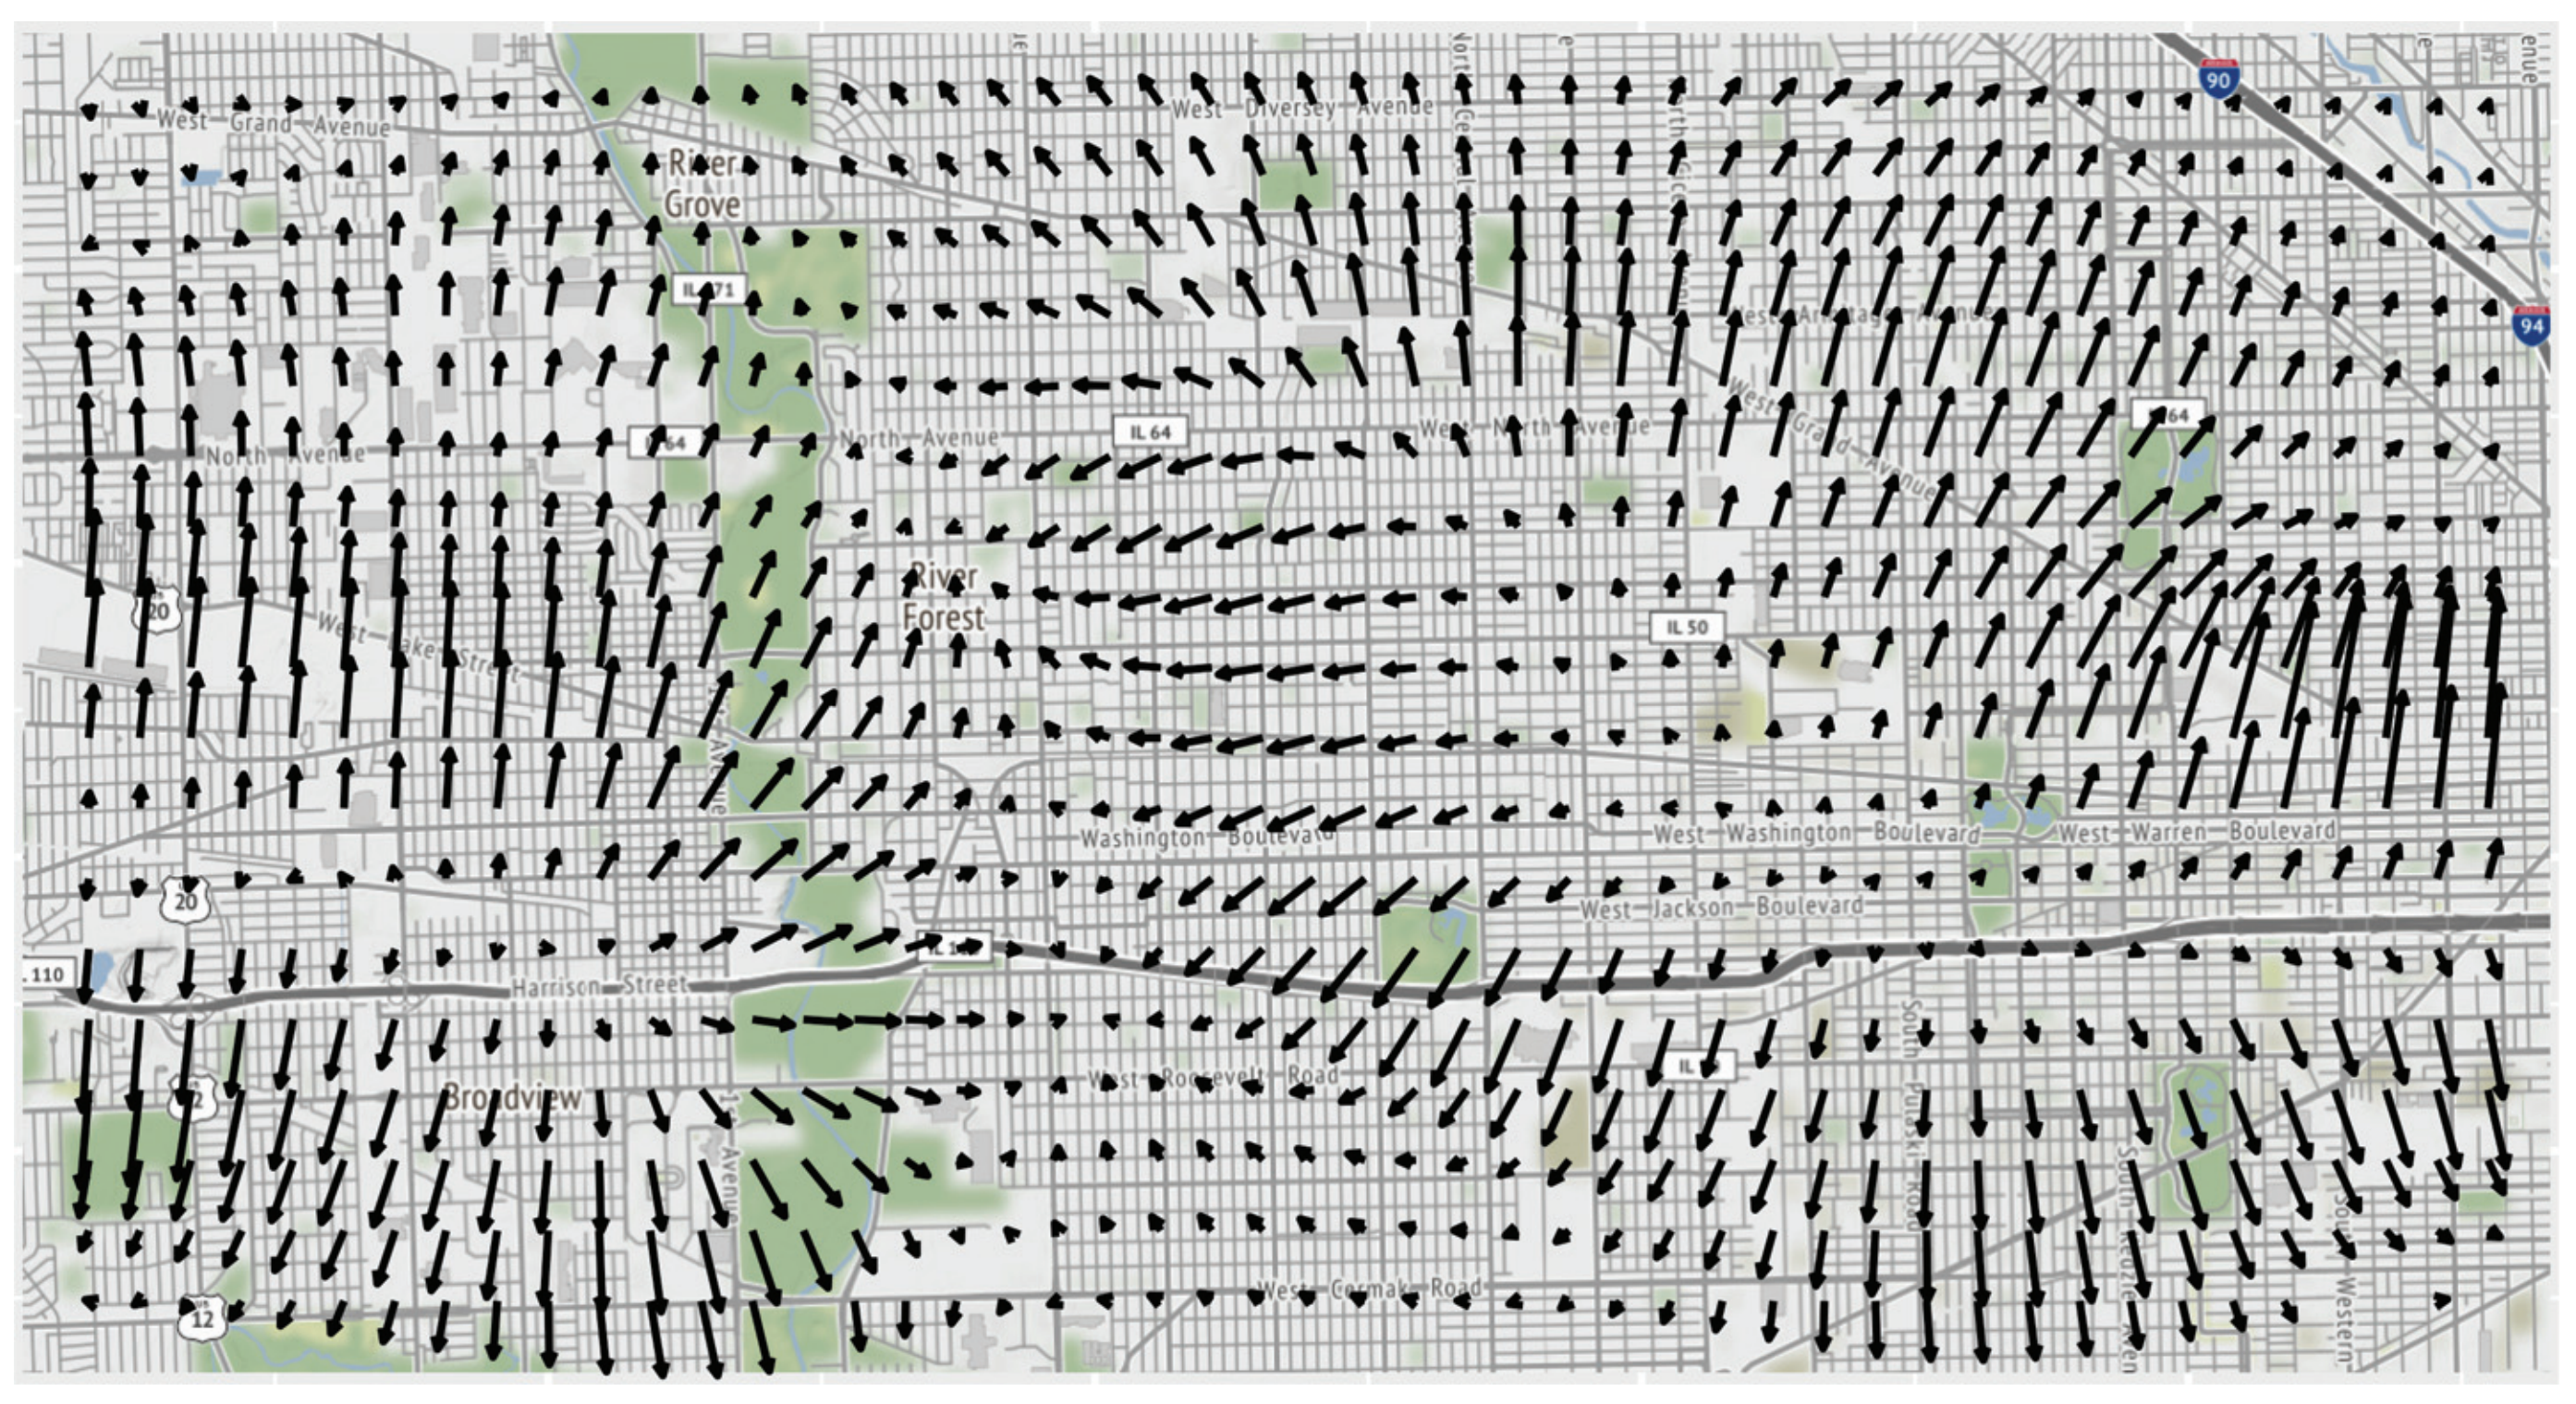
\includegraphics{chicagowest.pdf}
  \caption{White/non-white segregation gradients in the near-west suburbs of Chicago.}
  \label{fig:chicagowest}
\end{figure}

\begin{figure}
  \includegraphics{sanfran1317.pdf}
  \caption{Gentrification in San Fransisco. Income segregation patterns have changed from 2013 (left) to 2017 (right). The contours enclose neighborhoods whose residents tend to have incomes below the county median. Some of these neighborhoods have been shrinking. Thicker contours represent starker divisions.}
  \label{fig:sanfran1317}
\end{figure}


\begin{thebibliography}{3}

\bibitem{harrisjohnson18}
Harris, R., Johnson, R. (2018). Measuring and modelling segregation---New concepts, new methods and new data. \textit{Environment and Planning B: Urban Analytics and City Science.} 45(6): 999--1002. doi:\href{http://dx.doi.org/10.1177/2399808318808889}{10.1177/2399808318808889}

\bibitem{reardonosullivan04}
Reardon, S., O'Sullivan, D. (2004). Measures of Spatial Segregation. \textit{Sociological Methodology.} 34: 121--162. doi:\href{http://dx.doi.org/10.1111/j.0081-1750.2004.00150.x}{10.1111/j.0081-1750.2004.00150.x}

\bibitem{wandjones11} Wand, M. P., Jones, M. C. (2011). \textit{Kernel smoothing}, London: Chapman \& Hall.

\end{thebibliography}

\end{document}
